% -*- mode: fundamental -*-

% ****************************************************************

\chapter{BSV: Finite State Machines (FSMs); \\
The Drum CPU}

\markboth{Ch \arabic{chapter}: FSMs (DRAFT)}{\copyrightnotice}

\setcounter{page}{1}
% \renewcommand{\thepage}{\arabic{page}}
\renewcommand{\thepage}{\arabic{chapter}-\arabic{page}}

\label{ch_FSMs}

% ****************************************************************

\section{RISC-V: The interface for the Drum and Fife CPU modules}

\label{Sec_CPU_Module_Skeleton_CPU_interface}

A clean, common interface allows us transparently to substitute the
Drum CPU module for the Fife CPU module and \emph{vice versa}.

By sharing a common interface between the Drum and Fife CPU
modules, we can easily substiute one for the other in the overall
system.  We now have all the pieces in place to describe the interface:

\index{Drum!CPU interface}
\index{Fife!CPU interface}

\begin{Verbatim}[frame=single, numbers=left]
interface CPU_IFC;
   interface FIFOF_O #(Mem_Req) fo_IMem_req;
   interface FIFOF_I #(Mem_Rsp) fi_IMem_rsp;

   interface FIFOF_O #(Mem_Req) fo_DMem_req;
   interface FIFOF_I #(Mem_Rsp) fi_DMem_rsp;
endinterface
\end{Verbatim}

The interface is simple:

\begin{tightlist}

\item A \verb|FIFOF_O| to carry memory requests instructions (out-bound
from the CPU to the memory);

\item A \verb|FIFOF_I| to carry memory responses containing
instructions (in-bound from memory to the CPU);

\item A \verb|FIFO_O| to carry memory requests from load/store
instructions (out-bound from the CPU to the memory);

\item A \verb|FIFOF_I| to carry corresponding load/store memory
responses (in-bound from memory to the CPU).

\end{tightlist}

% ****************************************************************

\section{RISC-V: A skeleton CPU module for Drum}

\label{Sec_CPU_Module_Skeleton_skeleton_CPU_module}

\index{RISC-V!Drum skeleton module}
\index{RISC-V!Fife skeleton module}
\index{Drum!Skeleton module}
\index{Fife!Skeleton module}

Here is a skeleton of the CPU module for Drum.  We will fill in
the missing pieces in subsequent chapters.

\begin{Verbatim}[frame=single, numbers=left]
(* synthesize *)
module mkCPU (CPU_IFC);
   // ================================================================
   // STATE

   // Paths to and from memory
   FIFOF #(Mem_Req) f_to_IMem   <- mkFIFOF;
   FIFOF #(Mem_Rsp) f_from_IMem <- mkFIFOF;
   FIFOF #(Mem_Req) f_to_DMem   <- mkFIFOF;
   FIFOF #(Mem_Rsp) f_from_DMem <- mkFIFOF;

   // The integer register-file
   RegFile #(XLEN)    gprs  <- mkRegFileFull;

   // The program counter
   Reg #(Bit #(XLEN)) rg_pc <- mkReg (0);

   // Inter-step registers
   Reg #(F_to_D)                     rg_F_to_D                  <- mkRegU;
   Reg #(D_to_RR)                    rg_D_to_RR                 <- mkRegU;
   Reg #(RR_to_EX_IALU)              rg_RR_to_EX_IALU           <- mkRegU;
   Reg #(RR_to_EX_DMem_Req)          rg_RR_to_EX_DMem_Req       <- mkRegU;
   Reg #(EX_DMem_Req_to_EX_DMem_Rsp) rg_EX_DMem_Req_to_EX_DMem_Rsp <- mkRegU;

   // ================================================================
   // BEHAVIOR

   ... // This section will code the dynamic "behavior" of the module
   ... // and will be discussed in the next chapter

   // ================================================================
   // INTERFACE

   // One of the sub-interfaces
   interface FIFOF_O #(Mem_Req) fo_IMem_req;
      method Bool notEmpty();
         return f_to_IMem.notEmpty;
      endmethod

      method t first();
         return f_to_IMem.first;
      endmethod

      method Action deq();
         f_to_IMem.deq;
      endmethod
   endinterface

   ... // and similarly for the fi_IMem_rsp sub-interface
   ... // and similarly for the fo_DMem_req sub-interface
   ... // and similarly for the fi_DMem_rsp sub-interface

endmodule

\end{Verbatim}

With the interface transformers discussed in
Section~\ref{Sec_interface_transfomers}, we can simplify the INTERFACE
section of our Drum CPU module just four lines:

% ----------------

\begin{Verbatim}[frame=single, numbers=left]
(* synthesize *)
module mkCPU (CPU_IFC);

   ... STATE and BEHAVIOR ...

   // ================================================================
   // INTERFACE

   interface fo_IMem_req = to_FIFOF_O (f_to_IMem);
   interface fi_IMem_req = to_FIFOF_O (f_from_IMem);
   interface fo_DMem_req = to_FIFOF_O (f_to_DMem);
   interface fi_DMem_req = to_FIFOF_O (f_from_DMem);
endmodule
\end{Verbatim}

% ****************************************************************

\section{Introduction}

So far, we have only been discussing pure combinational functions, for
which there is no concept of time.  Combinational functions are just
``instantaneous'', pure mathematical functions transforming input
values to output values.  However, a CPU, as shown in
Figure~\ref{Fig_FSMs_Simple_Instr_Exec}
\begin{figure}[htbp]
  \centerline{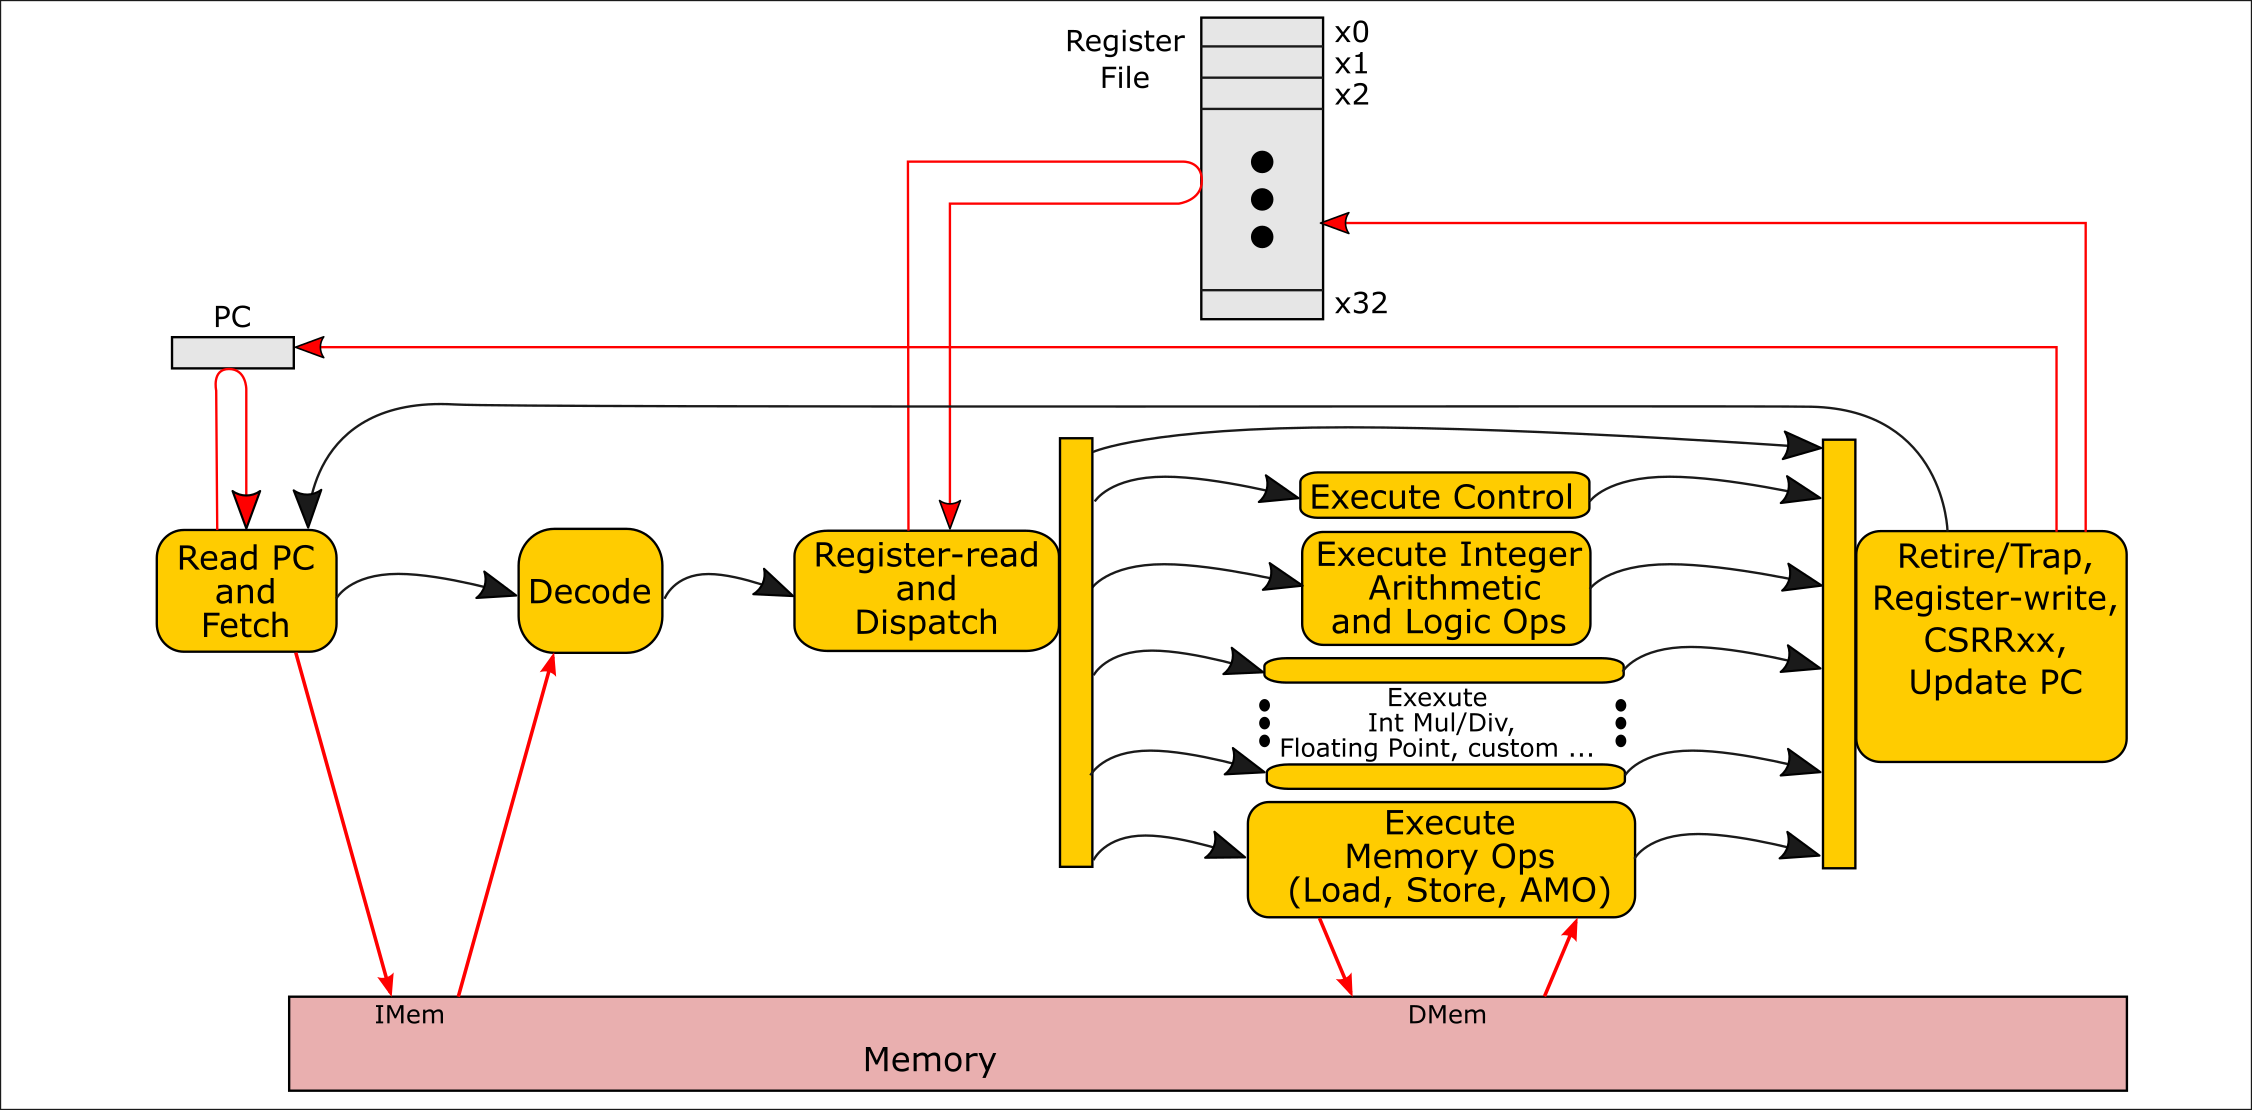
\includegraphics[width=6in,angle=0]{ch030_RISCV_Design_Space/Figures/Fig_Instr_Exec}}
  \caption{\label{Fig_FSMs_Simple_Instr_Exec}Simple interpretation of RISC-V instructions (same as Fig.~\ref{Fig_Instr_Exec})}
\end{figure}
represents a \emph{processs}, a behavior that evolves over time.  For
example the Drum CPU executes one full instruction after another,
and the black arrows in the diagram reprsent an infinite loop. For
each instruction, first it performs a Fetch operation, which sends a
request to memory. Some time later, the memory sends back a response,
which is then processed by the Decode step, before proceeding to the
next step, and so on.  After the Execute Control and Register-write
steps it loops back to the Fetch step for the next instruction.

In the Fife CPU, on the other hand, each of the yellow boxes
represents a ``stage'' and the black arrows represent messages sent
from one stage to another.  Each stage is itself an infinite loop,
consuming incoming messages and producing outgoing messages.  Thus,
while the Decode state is working on the first instruction, the Fetch
stage is already working on the second instruction, and so on.  There
is a sequence of instructions in this pipeline, advancing on every
``tick''.  A pipelined CPU also needs some additional state to manage
interactions between multiple instructions in the pipeline, such as
``epochs'', ``scoreboards'' and ``store-buffers'' (see
Figure~\ref{Fig_Instr_Exec_w_FIFOs}).

In this chapter we build up to creating the Drum CPU.

% ****************************************************************

\section{BSV: Finite State Machines (FSMs)}

\label{Sec_FSMs_FSMs}

\index{BSV!FSMs}
\index{BSV!Finite State Machines}

Finite state machines (FSMs) are a classical concept in digital
hardware design.  An FSM is an artefact that can, at any time, be in
one of of a number of possible \emph{states}.  One state is often
distinguised as the \emph{start} state, the initial state of the FSM.

From each state, an FSM can \emph{transition} to another state; the
choice of destination state may depend on predicates on the current
state and on external inputs to the FSM.

One classical notation for FSMs is ``bubble-and-arrow'' diagrams:
bubbles represent states, and arrows represent transitions between
states.  Thus, an FSM is a specification of a \emph{process} that,
over time, moves from state to to state.  The process can be infinite,
with an transitions back to earlier states.

\index{Drum!as an FSM}

For Drum, we will interpret
Figure~\ref{Fig_FSMs_Simple_Instr_Exec} as a bubble-and-arrow diagram
for an FSM.  Each of the yellow boxes will be a state, and the black
arrows represent state-transitions.

% ================================================================

\subsection{Sequential FSMs, Concurrent FSMs, and Digital Hardware}

\index{BSV!FSMs!sequential {\vs.} concurrent}
\index{BSV!FSMs!concurrent {\vs.} sequential}

Classical FSMs in the literature are \emph{sequential} FSMs---every
transition is from the current state to a unique, particular next
state.\footnote{The transition can be \emph{non-deterministic} in
choice of next-state from a set of states, but once the choice is
made, the FSM is again in a particular state}.

Most non-trivial digital hardware systems are \emph{concurrent FSMs}.
Different module instances are separate FSMs, each running their own
process(es).  These separate FSMs may communicate with each other
{\via} shared state (registers, fifos, register files, {\etc}).

\index{Fife!as a set of concurrent FSMs}

For Fife, we will interpret Figure~\ref{Fig_FSMs_Simple_Instr_Exec} as
a set of concurrent FSMs.  Each of the yellow boxes will be an FSM,
and the black arrows represent communication between FSMs.

% ****************************************************************

\section{BSV: {\tt StmtFSM}}

\label{Sec_FSMs_StmtFSM}

\index{BSV!StmtFSM@{\tt StmtFSM}}

The central BSV construct for temporal behavior (processes) is the
``\verb|rule|''.  Collections of rules can express any sequential or
concurrent FSM.  However, because Drum is a simple, structured
sequential process, we can use a simpler, higher-level BSV notation
called``\verb|StmtFSM|'' (which, in turn, is just converted into rules
by the \emph{bsc} compiler).

\verb|StmtFSM| is a sub-language within BSV for expressing
\emph{structured}, mostly sequential processes.\footnote{{\tt StmtFSM}
can also express structured fork-join parallelism, but we do not need
that for Drum.}  The constructs are similar to most common
sequential programming languages: blocks to express temporally
sequenced actions, if-then-elses, while-loops and for-loops.

(Note: we already briefly encountered a simple \verb|StmtFSM|---the
testbench in Section~\ref{BSV_small_testbench}.)

% ================================================================

\subsection{BSV: Actions and the {\tt Action} type}

\index{BSV!Action@{\tt Action}: primitive type of actions}
\index{BSV!actions}

The fundamental building-block for \verb|StmtFSM| is the ``action'',
which is a statement/expression of type \verb|Action|.  Some common
examples:

\begin{Verbatim}[frame=single, numbers=left]
   rg_pc <= rg_pc + 4;          // Assignment to a register
   f_F_to_D.deq;                // Dequeue a fifo
   f_D_to_RR.enq (v);           // Enqueue into a fifo
   $display ("Hello, World!");  // Print something (in simulation only)
\end{Verbatim}

As discussed in
Section~\ref{Sec_Register_syntactic_shorthands}
the first assignment statement is syntactic shorthand for:

\begin{Verbatim}[frame=single, numbers=left]
   rg_pc._write (rg_pc._read + 4)
\end{Verbatim}

{\ie} it is an invocation of the register \verb|_write| method which,
as described in
Section~\ref{Sec_Register_interface} has type
\verb|Action|.  Similarly, as described in
Section~\ref{Sec_FIFOF_interface}, fifo \verb|enq|
and \verb|deq| methods have return-type \verb|Action|, so the
statements \verb|f_D_to_RR.enq (v)| and \verb|f_D_to_RR.enq (v)| have
type \verb|Action|.

\index{BSV!display@{\tt \$display} has {\tt Action} type}

\verb|$display()| is a built-in construct in BSV that also has type
\verb|Action|.

% ----------------------------------------------------------------

\subsubsection{BSV: Action-blocks: grouping actions into larger actions}

The \verb|Action| type is recursive: it is either a primitive action
(like those described just above), or it is a collection of things of
type \verb|Action|, collected using an \verb|action| block (bracketed
by the BSV keywords \verb|action| and \verb|endaction|).  For example
the above primitive actions can be collected into a single entity
which itself has type \verb|Action|:

\begin{Verbatim}[frame=single, numbers=left]
   action
      rg_pc <= rg_pc + 4;          // Assignment to a register
      f_F_to_D.deq;                // Dequeue a fifo
      f_D_to_RR.enq (v);           // Enqueue into a fifo
      $display ("Hello, World!");  // Print something (in simulation only)
   endaction
\end{Verbatim}

Although the actions in an \verb|action| block must be written in some
textual order, there is no temporal ordering of these actions.  All
the primitive actions in an \verb|action| block (either directly in
the block or, recursively in a sub-block) occur ``instantly'' and
``simultaneously''.

% ================================================================

\subsection{BSV: {\tt StmtFSM}: sequences of actions}

\index{BSV!StmtFSM@{\tt StmtFSM}!seq@{\tt seq .. endseq}: sequences of actions}

Our first construct that has temporal behavior is the
\verb|seq|-\verb|endseq| block.  Each item in the block is typically
an entity of type \emph|Action|, and they are performed sequentially,
one after another.

The testbench in Section~\ref{BSV_small_testbench} contains an example
of a \verb|seq| block:
\begin{Verbatim}[frame=single, numbers=left]
      seq
         ... action 1 ...

         ... action 2 ...

         ... action 3 ...

         ... action 4 ...
      endseq
\end{Verbatim}

\index{BSV!FSMs!Stmt@{\tt Stmt}: type of argument to FSM module constructors}

The \verb|seq| block itself has type \verb|Stmt|.  The items in a
block can have type \verb|Action| or the type \verb|Stmt|, {\ie},
blocks can be nested.

% ================================================================

\subsection{BSV: {\tt StmtFSM}: if-then-elses}

\index{BSV!StmtFSM@{\tt StmtFSM}!if@{\tt if-then-else}: conditional actions}

Conditional execution can be expressed with traditional if-then-else notation:
\begin{Verbatim}[frame=single, numbers=left]
   if ... Bool expression ...
      ... expression of type Stmt ...
   else
      ... expression of type Stmt ...
\end{Verbatim}

Note: in Section~\ref{BSV_Combo_Circuits_if_then_else} we described
ordinary BSV if-then-else expresions.  \verb|StmtFSM| uses the same
notation, but there is no ambiguity---the context always clearly
distinguishes what we mean, because there is no overlap between
ordinary expressions and \verb|StmtFSM| constructions.

% ================================================================

\subsection{BSV: {\tt StmtFSM}: while-loops}

\index{BSV!StmtFSM@{\tt StmtFSM}!while@{\tt while}: loop-repetition of actions}

Repetitive processes can be expressed with traditional while-loop notation:
\begin{Verbatim}[frame=single, numbers=left]
   while (... Bool expression ...)
      ... expression of type Stmt ...
\end{Verbatim}

(Note: \verb|StmtFSM| also has for-loop notation, but we do not need it for Drum.)

% ================================================================

\subsection{BSV: {\tt StmtFSM}: {\tt mkAutoFSM}: a simple FSM module constructor}

\index{BSV!StmtFSM@{\tt StmtFSM}!{\tt for}: loop-repetition of actions}

Given an entity of type \verb|Stmt|, we can pass it as an argument to
to the module constructor \verb|mkAutoFSM|

\begin{Verbatim}[frame=single, numbers=left]
   mkAutoFSM (... expression of type Stmt ...);
\end{Verbatim}

This creates an FSM with the behavior specified by the \verb|Stmt|
argument.  The FSM starts running immediately as we come out of reset,
starting at the first statement, and terminates when we fall through
the last statement.

% ****************************************************************

\section{RISC-V: The Drum CPU module}

\label{Sec_FSMs_Drum_CPU_module}

\index{RISC-V!Drum CPU module}
\index{Drum!CPU module}

The outline of the CPU module for Drum was shown in the display in
Section~\ref{Sec_CPU_Module_Skeleton_skeleton_CPU_module}.  Here we
fill in the BEHAVIOR section that we elided in that display.

\begin{Verbatim}[frame=single, numbers=left]
(* synthesize *)
module mkCPU (CPU_IFC);

   // ================================================================
   // STATE

   ... // shown earlier

   // ================================================================
   // BEHAVIOR

   mkAutoFSM (
      seq
         fa_Fetch_step;
         fa_Decode_step;
         fa_Register_Read_and_Despatch_step;

         if (rg_D_to_RR.opclass == OPCLASS_ILLEGAL) action
	    $display ("%0d: RR.rl_RR: ILLEGAL INSTR", cur_cycle);
	    $display ("  ", fshow_D_to_RR (x));
	    $finish (1);
         endaction

	 else if (result_RR.redirect)
	    rg_pc <= y.redirected_pc;

	 else if (result_RR.to_RW.merge_source == MERGE_EX_IALU) seq
	    rg_RR_to_EX_IALU <= result_RR.to_EX_IALU;
            fa_EX_IALU_step;
	    fa_RR_to_RW_step;

	 else if (result_RR.to_RW.merge_source == MERGE_EX_MEM)
            f_to_DMem.enq (result_RR.to_DMem);
            fa_EX_Mem_step;
	    fa_RR_to_RW_step
      endseq);

   // ================================================================
   // INTERFACE

   ... // shown earlier
endmodule

\end{Verbatim}

% ****************************************************************

\section{RISC-V: Compiling Drum BSV code to Verilog}

\label{Sec_FSMs_Drum_compile_to_verilog}

% ****************************************************************

\section{RISC-V: Compiling and linking Verilog using Verilator}

\label{Sec_FSMs_Drum_verilator}

% ****************************************************************

\section{RISC-V: Verilog simulation of Drum}

\label{Sec_FSMs_Drum_simulation}

% ****************************************************************

\section{RISC-V: Implementing Drum Verilog on an FPGA}

\label{Sec_FSMs_Drum_FPGA}

% ****************************************************************
